\documentclass[a4paper]{article}
\usepackage[spanish]{babel}
\usepackage[utf8]{inputenc}

\usepackage{caratula}
\usepackage{graphicx}

\usepackage{hyperref}

\usepackage{subcaption}

\usepackage{algorithm}
\usepackage{algpseudocode}

\usepackage{fancyhdr}
\pagestyle{fancy}

\fancyhf{}

\fancyfoot[RO]{\thepage}
\renewcommand{\headrulewidth}{0.5pt}
\renewcommand{\footrulewidth}{0.5pt}
\setlength{\hoffset}{-0.8in}
\setlength{\textwidth}{16cm}
\setlength{\headsep}{0.5cm}
\setlength{\textheight}{25cm}
\setlength{\voffset}{-0.7in}
\setlength{\headwidth}{\textwidth}
\setlength{\headheight}{13.1pt}

\renewcommand{\baselinestretch}{1.1}  % line spacing

\begin{document}

	\materia{Organización del computador II}
	\titulo{TP Final: Generación de terrenos montañosos por elevación}
	\integrante{Florencia Zanollo}{934/11}{florenciazanollo@gmail.com}
	\integrante{Luis Toffoletti}{827/11}{luis.toffoletti@gmail.com}
	
	\maketitle
	
	\tableofcontents
	\newpage

	\section{Introduccion}

Para este trabajo práctico nos propusimos implementar el modelo para generación de terreno explicado en el paper "The Uplift Model Terrain Generator".\footnote{\url{https://www.dropbox.com/s/q6brk3jqwppxrhx/upliftTerrainGenerator.pdf?dl=0}}

En él se propone la generación de terreno montañoso a partir de elevaciones o picos. El modelo se puede aplicar tanto en 2D como 3D. La idea general del algoritmo es generar picos de manera aleatoria y luego obtener la altura final de cada porción del terreno promediando las influencias provenientes de las elevaciones.

Realizaremos dos implementaciones del modelo, una de ellas en C++ y la otra en ASM utilizando la tecnología SIMD. Nuestro objetivo es comparar estas implementaciones y ver si nuestro código ASM es más veloz que el generado por el compilador (g++).
	\newpage
	
	\section{Implementación}

El método requiere de los siguientes datos de entrada:
\begin{description}
\item[divisions] cantidad de divisiones sobre la cuál se colocarán los picos.
\item[nroPeaks] cantidad total de picos.
\item[yMin] altura mínima permitida de un pico.
\item[yMin] altura máxima permitida de un pico.
\item[ruggedness] escabrosidad del terreno, es decir, qué tanto afecta un pico a sus posiciones aledañas.
\end{description}
\smallskip

Lo que denominamos '\textbf{pico}', es un valor que será generado y ubicado aleatoriamente ocupando alguna de las posiciones posibles (divisions). Representa un punto de elevación en el terreno que luego el algoritmo se encargará de interpretar (en conjunto con la información del resto de los picos) para definir el valor definitivo que tendrá la elevación en cada punto del terreno.
\begin{figure}[h]
\centering
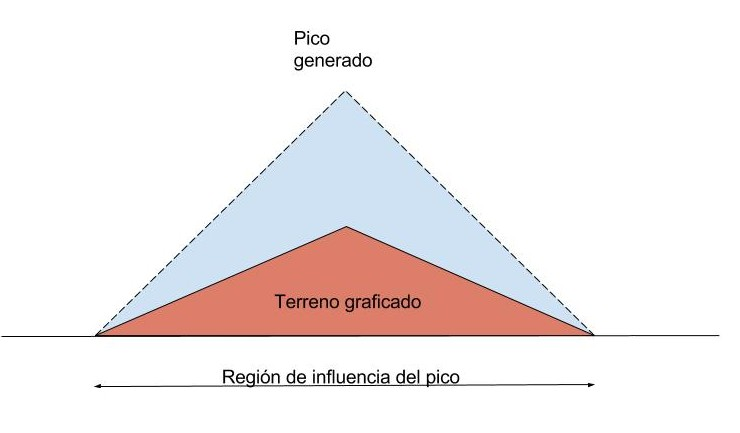
\includegraphics[width=0.7\linewidth]{imagenes/Pico1}
\caption{}
\label{fig:Pico1}
\end{figure}
\begin{figure}[h]
	\centering
	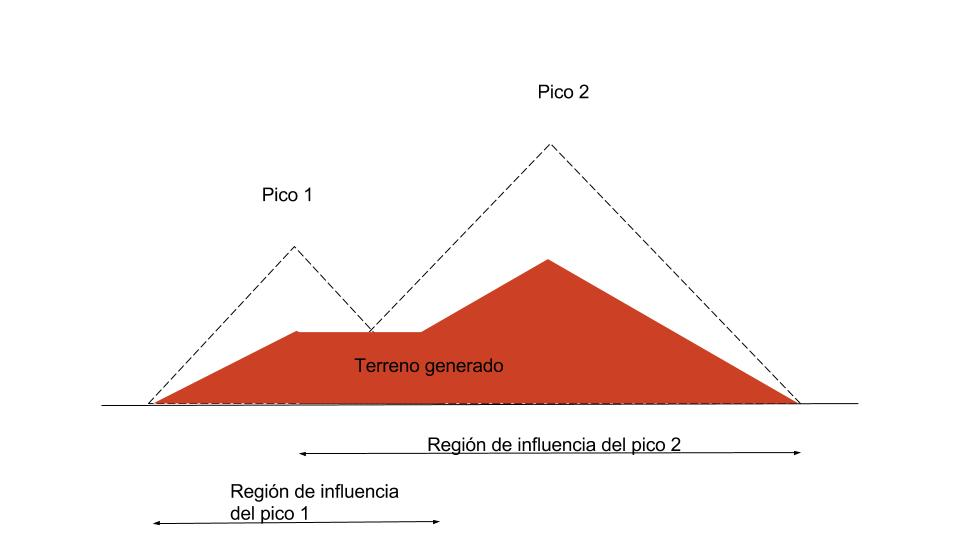
\includegraphics[width=0.7\linewidth]{imagenes/pico2}
	\caption{}
	\label{fig:pico2}
\end{figure}

En la figura 1 podemos ver un terreno generado a partir de un único pico, como se puede apreciar el valor del pico se promedia con el suelo para obtener el terreno definitivo. Se observa también una zona de influencia del pico, es aquella en la cual el punto de elevación afecta en el cálculo final del terreno.


El concepto de '\textbf{influencia}' de un pico podemos visualizarlo mejor en la figura 2. El terreno fue generado a partir de dos picos, existe una región  donde tenemos influencia por parte de ambos, es donde se forma una meseta ya que el algoritmo promedia la altura que tienen los picos en esa región. En el resto del terreno hay influencia de un sólo pico o ninguno.

En nuestro caso también contamos con las siguientes entradas, las cuáles agregamos por razones de utilidad a la hora de experimentar y comparar las implementaciones de C y ASM.
\begin{description}
\item[seed] permite setear una semilla particular para el random, esto es para lograr el mismo gráfico y poder experimentar con datos más certeros.
\item[debugging] si una semilla es proporcionada entonces se le puede decir al programa que entre en modo verbouse; el cuál nos va a dar, además del gráfico, el valor numérico de cada posición del terrreno final y la posición y tamaño original de cada pico.
\end{description}
\smallskip

Para poder llevar a cabo el método vamos a estar utilizando las siguientes estructuras:
\begin{description}
\item[peaksPos] arreglo con nroPeaks posiciones, cada una contiene la posición dentro del terreno de dicho pico. Las posiciones van de 0 a divisions-1.
\item[peaksSize] arreglo con nroPeaks posiciones, cada una contiene la altura de dicho pico. Las alturas posible están entre yMin e yMax (inclusive en ambos casos).
\item[terrain] vector con los valores numéricos finales de cada posición del terreno.
\end{description}
\smallskip

Los picos son generados de manera aleatoria, tanto su posición como su altura (dentro de los límites explicados más arriba). Luego se hace lo siguiente:

\begin{algorithm}
\begin{algorithmic}

\ForAll{divisions} 
	\ForAll{peaks} 
		\Comment{se calcula la influencia de cada pico para cada posición}
		\State influencia $\gets$ altura del pico - distancia del pico a la posición actual * ruggedness.
	\EndFor
	
	\If{la posición no tiene influencia de nadie} 
		\State valor final de la posición $\gets$ 0.
	
	\ElsIf{la posición solo es influenciada por un pico} 
		\State valor final de la posición $\gets$ influencia / 2.
	
	\ElsIf{la posición es influenciada por dos o más picos}
		\State valor final de la posición $\gets$ influencia / cantidad de picos con influencia sobre ella.
		
	\EndIf

\EndFor

\end{algorithmic}
\end{algorithm}

Quedando así en cada posición del terreno final el valor de 'promediar' todos los picos que tienen influencia sobre ella.

La complejidad teórica del algoritmo es $\theta(divisions*peaks)$ ya que indefectiblemente se recorren ambos y el resto de las operaciones son $O(1)$.

\subsection{Versión de C}
Está versión es muy sencilla ya que se puede mapear directamente el pseudocódigo a código, con pocas modificaciones. Luego basta con compilar utilizando las mejoras de sse para contar con las herramientas de SIMD.

\subsection{Versión de ASM}
La idea es simple, recorrer las posiciones del terreno de a cuatro, ya que como cada una es un float esa es la cantidad que entran en un registro xmm. 
Luego, en cada iteración, recorrer todos los picos, también de a cuatro (son int pero de 32 bits, es decir, cuatro por registro xmm).

Cuando obtenemos los datos de los picos, expandimos y repetimos la información de cada uno en distintos registros. 
Para que la explicación sea más clara mostraremos el caso del pico uno (P1) siendo los demás prácticamente iguales salvo por la información a usar. Entonces:\\

Primero se replica la posición actual en un registro xmm, al cuál le sumamos un registro constante con los enteros 0 a 3, es decir, nos queda el valor de cada una de las cuatro posiciones que estamos calculando en cada entero.

\begin{center}
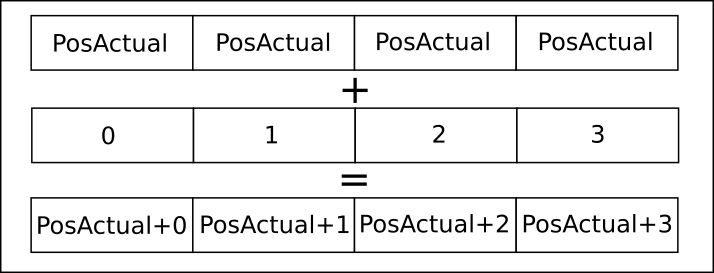
\includegraphics[scale=0.5]{imagenes/posActual.png} 
\end{center}

Luego, tanto para la posición (Pos) como para la altura (Size) de P1, se crean registros con la información replicada en cada int.

\begin{center}
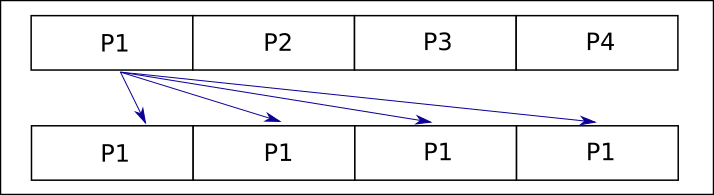
\includegraphics[scale=0.5]{imagenes/P1replicaInfo.png} 
\end{center}

Contamos con dos acumuladores, uno para la 'influencia' de los picos en esa posición y otro para la cantidad de picos que influyen. Para calcular el primero realizamos lo siguiente, donde Abs hace referencia a la función de valor absoluto:

\begin{center}
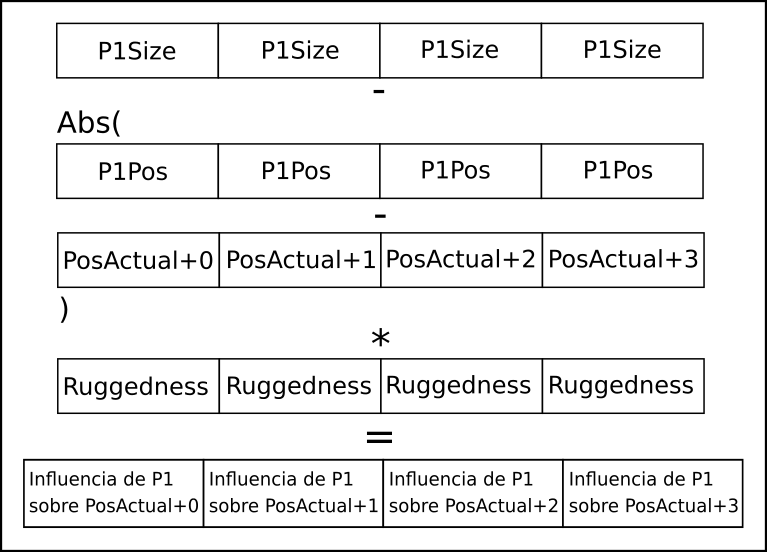
\includegraphics[scale=0.5]{imagenes/calculoInfluencia.png} 
\end{center}

Utilizando el registro que contiene la influencia obtenemos si el pico influye (influencia $>$ 0) o no (caso contrario) sobre cada una de las cuatro posiciones.

Sumando esta información para cada pico obtenemos cuánta influencia, y de cuántos picos, tiene una posición determinada. Así al final del ciclo que recorre los picos solo nos queda dividir influencia por cantidad de picos y así obtenemos el valor real del terreno en la posición.

	\newpage
	
	\section{Experimentación y Resultados}

Al experimentar siempre es de suma importancia elegir los casos de prueba. Como es un algoritmo que depende de una semilla random lo primero que decidimos fue dejarla fija, para que las sucesivas ejecuciones fuesen de la misma naturaleza. El algoritmo es de complejidad lineal respecto de divisiones por cantidad de picos, por ende al experimentar probamos diferentes combinaciones de los mismos.\\

Basandonos solo en la teoría, en un comienzo suponíamos una mejora en la performance de ASM cercana a 16 veces la de C. Llegamos a ese número partiendo de que, si C no tenía ninguna mejora iba a poseer la complejidad teórica de divisiones por cantidad de picos; mientras que nuestro ASM recorría tanto las divisiones como los picos de a cuatro, si consideramos esto nos queda $divisiones/4 * picos/4$. Esta complejidad es del mismo orden de grado (lineal) modificada solo por la constante $1/16$, presentando así una mejora del 93.75$\%$.\\

Para la recolección de datos utilizamos la librería Nonius\footnote{\url{https://nonius.io/}} que toma varias muestras, corriendolas muchas veces y procesa los resultados eliminando outliers. Las pruebas fueron corridas sobre un procesador Intel$^{®}$ Core™ i5-6200U\footnote{\url{https://ark.intel.com/es-es/products/88193/Intel-Core-i5-6200U-Processor-3M-Cache-up-to-2_80-GHz}}.\\

Los datos con los que fueron generados los gráficos se encuentran la siguiente url \url{http://cor.to/OrgaIIDatos} y los gráficos se encuentran de manera interactiva en las url al pie de la página de cada uno.

\subsection{Misma cantidad de picos, distintas divisiones}
Como primer experimento fijamos la cantidad de picos y fuimos aumentando las divisiones.

\centerline{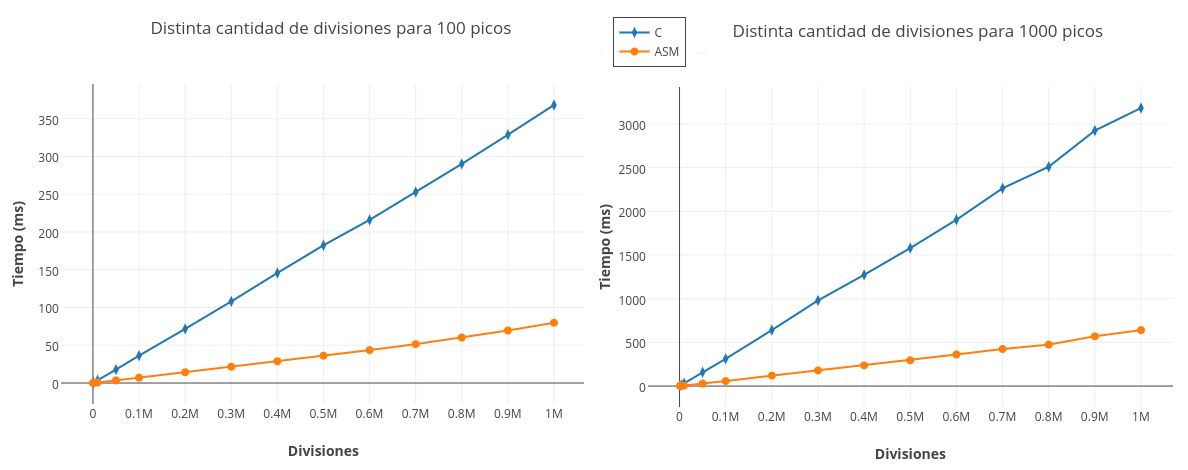
\includegraphics[scale=0.45]{imagenes/distintasDivisionesParaPicos.png}}\footnote{ 100 picos: \url{https://plot.ly/~fzanollo/55/} 1000 picos: \url{https://plot.ly/~fzanollo/53/}} 

En el gráfico de la izquierda probamos con 100 picos, como se ve al aumentar las divisiones el tiempo consumido crece de forma lineal. Si bien se presenta una mejora promedio del 78$\%$, no alcanza a los valores teóricos esperados.

En el de la derecha con 1000 picos. A pesar de que el gráfico muestra la misma tendencia analizando los datos encontramos que ahora la mejora es un poco más notoria y se eleva al 81$\%$.

\newpage

\subsection{Misma cantidad de divisiones, distinto porcentaje de picos}

El siguiente conjunto de casos de prueba fueron con una cantidad fija de divisiones, variando el porcentaje de picos respecto a las mismas.\\

Estos gráficos resultaron muy parecidos entre sí y respecto al anterior conjunto de pruebas. 

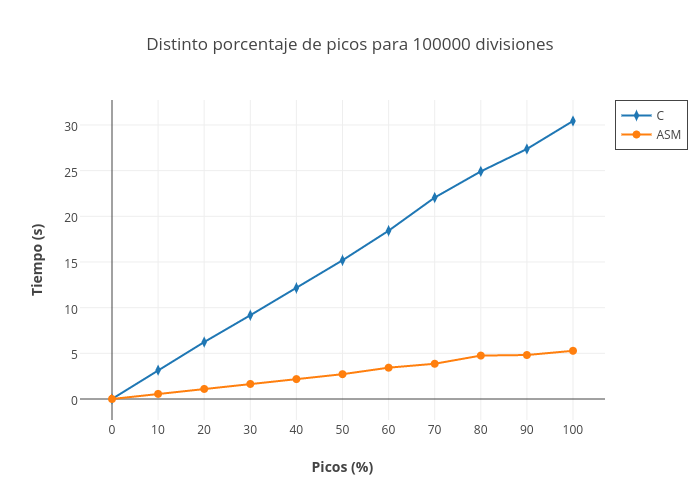
\includegraphics[scale=0.6]{imagenes/distintosPicos100000divisiones.png}\footnote{ 100000 divisiones: \url{https://plot.ly/~fzanollo/51/}}  

A medida que se aumentan las divisiones el gráfico se asemeja más al de una función lineal ya que se obtienen resultados más fehacientes.\\

Esto es porque, normalmente, a la hora de medir cantidad de ciclos de CPU pueden suceder diferentes eventos que alteran las mediciones, el ruido generado por los eventos se notan más si son pocos ciclos.

\centerline{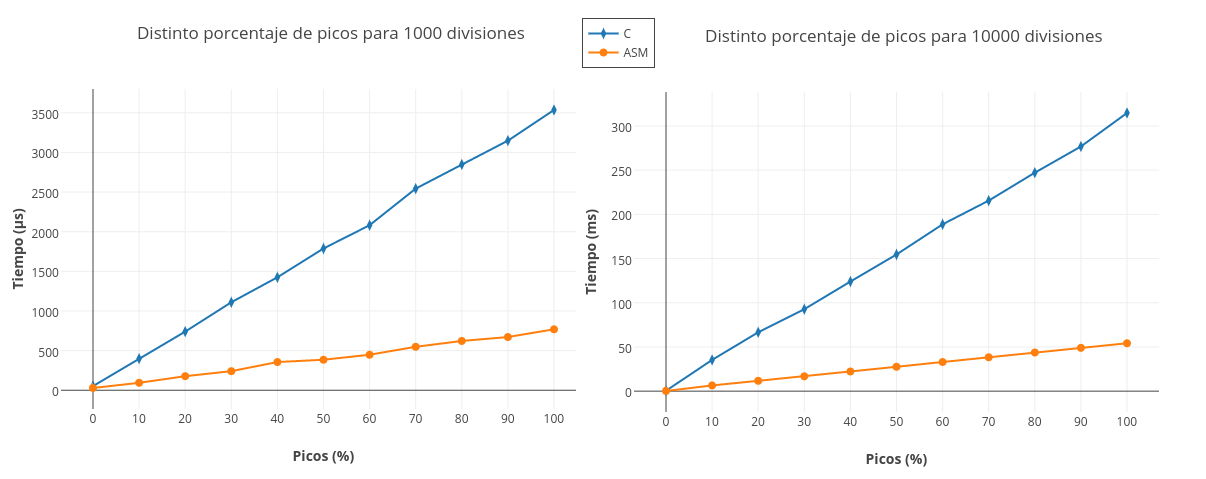
\includegraphics[scale=0.45]{imagenes/distintosPicosParaDivisiones.png}}\footnote{ 1000 divisiones: \url{https://plot.ly/~fzanollo/61/} 10000 divisiones: \url{https://plot.ly/~fzanollo/59/}} 

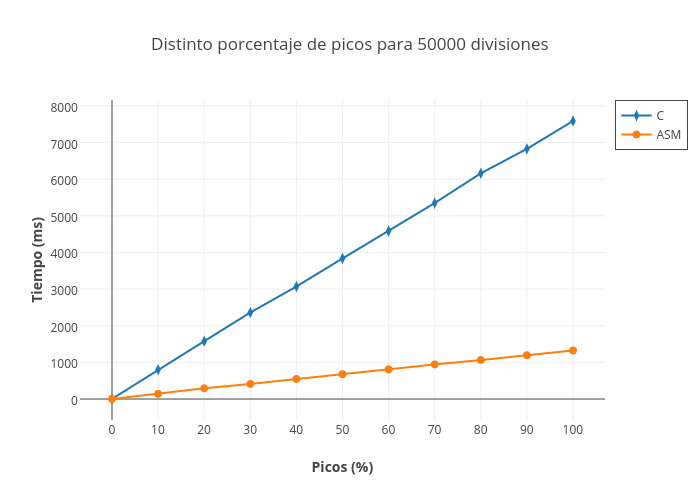
\includegraphics[scale=0.6]{imagenes/distintosPicos50000divisiones.png} \footnote{ 50000 divisiones: \url{https://plot.ly/~fzanollo/57/}} 

Dado que eran muy parecidos decidimos presentar los casos más chicos (1000 y 10000 divisiones) conjuntamente. La mejora promedio aproximada entre todos estos casos de prueba es del 80$\%$.

\newpage
\subsection{Misma cantidad de tamaño de entrada}

En los casos de prueba que listamos previamente mantuvimos fija una variable (cantidad de picos o cantidad de divisiones) e incrementamos la restante, como complemento realizamos un análisis manteniendo el tamaño total fijo, lógicamente la cantidad de picos no puede superar a la de divisiones.
Cantidad de picos p x Cantidad de divisiones d = Tamaño de entrada total T

En principio pensamos que el tiempo de ejecución debería mantenerse en todos los casos, debido a que tienen la misma complejidad teórica. En todo caso aumentando ligeramente para los casos con mayor cantidad de picos, debido a los cálculos previos para obtener los datos aleatorios de las ubicaciones y tamaños.

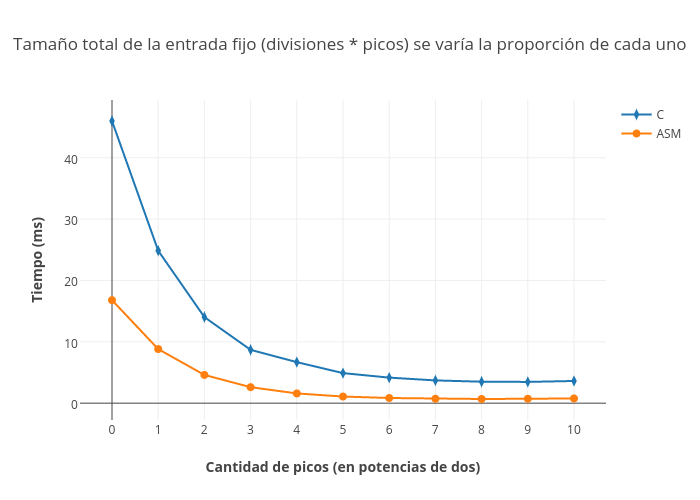
\includegraphics[scale=0.6]{imagenes/tamanioTotalFijo.png} \footnote{ Tamaño total fijo: \url{https://plot.ly/~fzanollo/63/}} 

Como vemos en el gráfico, a medida que crece el número de picos y disminuye la cantidad de divisiones, el tiempo de procesamiento decrece.\\

Obtuvimos un grupo de casos, desde un pico con 1024x1024 divisiones hasta 8 picos con 1024x128 divisiones (en el gráfico desde 0 hasta 3), que presenta un comportamiento diferente al resto en cuanto a tiempo de procesamiento.

Si bien estos casos podrían analizarse en profundidad, vamos a descartarlos ya que poseen un porcentaje de picos muy bajos para una generación de terreno concreta (mucho menos del 1$\%$).\\

Para el resto de los casos donde los porcentajes de picos sobre divisiones son más considerables, las gráficas se observan más estables.
	\newpage	
	
	\section{Conclusión}


\subsection{Mejoras}
Si se tiene en cuenta los valores máximos de cada división se podría llegar a utilizar enteros de menor tamaño para poder procesar de a más cantidad de datos. Por ejemplo si se usan enteros de 2Bytes se puede procesar hasta de a ocho por registro xmm.

Se podría hacer la versión 3D. La complejidad en cuanto al algoritmo e implementación no es muy elevada, sí nos pareció complicado dibujar el terreno generado, ya que deberíamos usar herramientas de SDL que no tenemos muy claras, por esa cuestión y la falta de tiempo para aprenderlas decidimos incluir en este trabajo solo la versión 2D.
	
\end{document}